%% -*- coding: utf-8; -*-

\documentclass[12pt,a4paper,oneside,english,spanish]{tesis} %% Llama a tesis.cls
\usepackage[utf8]{inputenc}
\usepackage[T1]{fontenc}
\usepackage[spanish, es-tabla]{babel} %% reemplaza "cuadro" por "tabla"
\usepackage{graphicx}
\usepackage{booktabs}
\usepackage{amssymb}
\usepackage{amstext}
\usepackage{float}
\usepackage{setspace}
\usepackage{listings}
\usepackage{color}
\usepackage{calc}
\usepackage{array}
\usepackage{textcomp}
\setcounter{secnumdepth}{3}
\setcounter{tocdepth}{3}

\graphicspath{{images/}}

%%%%%%%%%  Silabeo de palabras:  %%%%%%%%%%%%
\hyphenation{con-fi-gu-ra-cio-nes}         %%
%%%%%%%%%%%%%%%%%%%%%%%%%%%%%%%%%%%%%%%%%%%%%

%%%%%%%%%%%% Comandos para reducir errores, pero si no se ponen igual se compila%%%%%%%%%%%%%%%%%%%%%
\makeatletter                               																											 %%
%%%%%%%%%%%%%%%%%%%%%%%%%%%%%% LyX specific LaTeX commands. 																			 %%
%% Because html converters don't know tabularnewline																			 				 %%
\providecommand{\tabularnewline}{\\} 																			 												 %%
\floatstyle{ruled}																			 																					 %%
\newfloat{algorithm}{tbp}{loa}[chapter]																			 											 %%
																			 																														 %%
%\floatname{algorithm}{Algorithm}																			 														 %%
\floatname{algorithm}{ } %Con esta linea ya no aparece Algorithm																	 %%
																			 																			 											 %%
\DeclareRobustCommand{\greektext}{%
  \fontencoding{LGR}\selectfont\def\encodingdefault{LGR}}
\DeclareRobustCommand{\textgreek}[1]{\leavevmode{\greektext #1}}
\DeclareFontEncoding{LGR}{}{}
\DeclareTextSymbol{\~}{LGR}{126}
\newcommand{\lyxmathsym}[1]{\ifmmode\begingroup\def\b@ld{bold}
  \text{\ifx\math@version\b@ld\bfseries\fi#1}\endgroup\else#1\fi}
  \makeatother

%%%%%%%%%%%%%%%%%%%%%%%%%%%%%% Textclass specific LaTeX commands.
\newenvironment{lyxcode}
{\par\begin{list}{}{
\setlength{\rightmargin}{\leftmargin}
\setlength{\listparindent}{0pt}% needed for AMS classes
\raggedright
\setlength{\itemsep}{0pt}
\setlength{\parsep}{0pt}
\normalfont\ttfamily}%
 \item[]}
{\end{list}}

\makeatother

\addto\shorthandsspanish{\spanishdeactivate{~<>}}
%%%%%%%%%%%%%%%%%%%%%%%%%%%%%%%%%%%%%%%%%%%%%%%%%%%%%%%%%%%%%%%%%%%%%%%%%%%%%%%%%%%%%%%%%%%%%%%%%%%%%

\hoffset -1in
\voffset -1in
\topmargin 0.5cm
\headheight 1cm
\headsep 1.5cm
\footskip 1cm
\oddsidemargin 4cm
\textwidth 14.5cm
\textheight 23.2cm
\parindent 5ex

\university{UNIVERSIDAD NACIONAL DE INGENIERÍA}
\faculty{FACULTAD DE INGENIERÍA MECÁNICA}
\title{Y}
\title{PLANIFICACIÓN DE TRAYECTORIAS PARA ROBOTS MÓVILES EN ENTORNOS NO DINÁMICOS EMPLEANDO EL ALGORITMO RRT}
\logo{uni_logo.png}
\degree{INGENIERO MECATRÓNICO}
\author{PAREDES MERINO, JORGE SALVADOR}
\promotion{2010-II}
\place{LIMA - PERÚ}
\date{2012}

\addto\captionsenglish{
\renewcommand\bibname{BIBLIOGRAFÍA}
\renewcommand\appendixname{APÉNDICE}
}


\begin{document}
\pagestyle{empty}
\maketitle
\null \vfil \vfil

\begin{center}
\textbf{Dedicatoria}
\end{center}
\vspace{0.5cm}
Dedico el presente trabajo a .......

\vfil \null
\newpage 

\null \vfil \vfil

\begin{center}
\textbf{Agradecimientos}
\end{center}
\vspace{1cm}
Quería agradecer .......

\vfil \null
\newpage


\renewcommand\contentsname{TABLA DE CONTENIDOS}
\renewcommand\listfigurename{LISTA DE FIGURAS}


\pagestyle{headings}
\pagenumbering{roman}
\tableofcontents
\listoffigures
\listoftables

\doublespacing
\newpage
\addcontentsline{toc}{chapter}{\hspace{14pt} \bf PRÓLOGO \hfill}
\null\vspace{2.55 cm}
\begin{center}
  {\large \bfseries PRÓLOGO}
\end{center}
\vspace{1cm}
\pagenumbering{arabic}
Este es el prólogo.....

% -*- coding: utf-8; -*-
\chapter{INTRODUCCIÓN}


\section{Antecedentes}

Ejemplo de referencia: ..... ver robot Shakey%
\footnote{Desarollado entre 1966 y 1972%
} (ver Figura \ref{Flo:shakey}, tomada de \cite{Greenia}).

%
\begin{figure}[H]
\begin{centering}
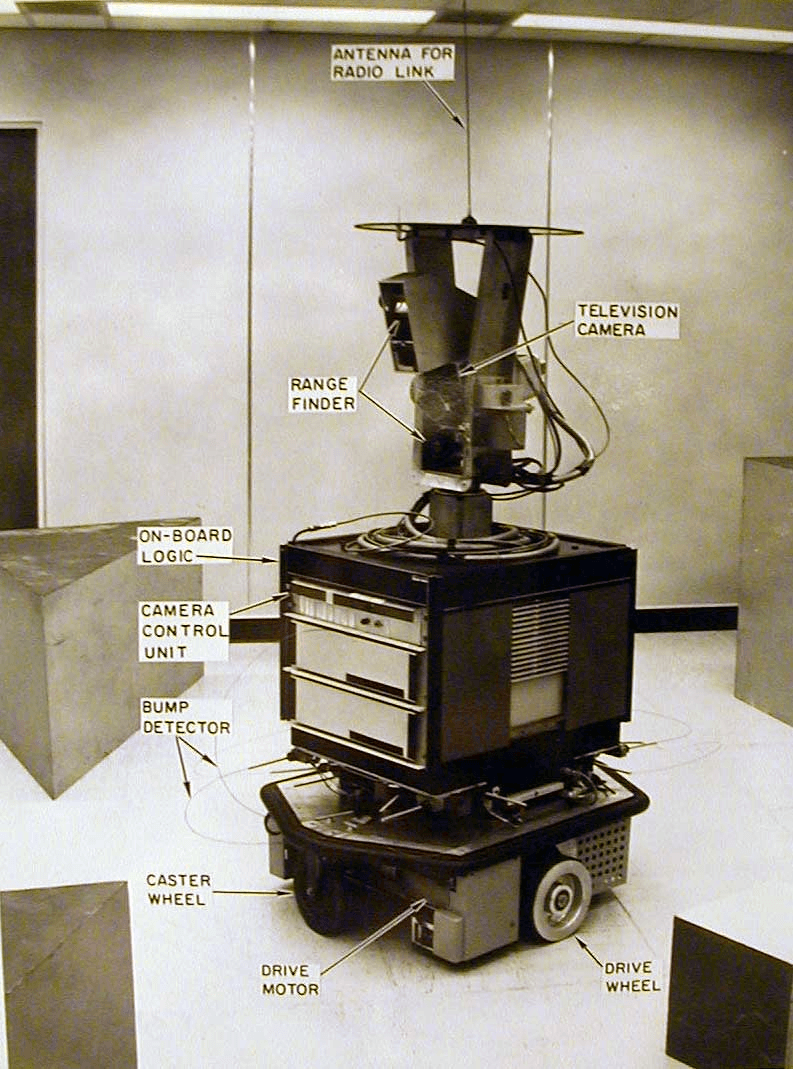
\includegraphics[scale=0.25]{Cap1/Shakey-the-Robot-SRI-1968}
\par\end{centering}

\caption{Robot Shakey(1968).}


\label{Flo:shakey}
\end{figure}

\section{Motivación de la investigación}


\section{Objetivos}


\section{Alcances}


\section{Limitaciones}

% -*- coding: utf-8; -*-
\chapter{ALGORITMO RRT}


\section{Elementos}



El algoritmo RRT original se basa en la construcción de un árbol de
configuraciones que crece buscando a partir de un punto origen. Para
entender el algoritmo se usará la nomenclatura expresada en el cuadro


% -*- coding: utf-8; -*-
\begin{table}[H]
\centering
\begin{tabular}{l>{\raggedright}p{4in}} \toprule
Elemento & \centering{}Descripción\tabularnewline\midrule
$C$ & es el conjunto de todas las configuraciones posibles del entorno,
es decir, los obstáculos y las configuraciones libres.\tabularnewline
$C_{free}$ & Subconjunto de C, configuraciones libres de obstáculos existentes.\tabularnewline
$R$ & Indicador de ponderación de proximidad al punto deseado. La distancia
euclidiana es la más utilizada.\tabularnewline
$q_{init}$ & Configuración inicial\tabularnewline
$q_{fin}$ & Configuración que se desea alcanzar\tabularnewline
$q_{rand}$ & Configuración aleatoria dentro del espacio $C_{free}$ \tabularnewline
$q_{near}$ & Es la conguración mas proxima a $q_{rand}$ , en el sentido denido
por R, de entre las existentes en un árbol. Se evalúa con el indicador
de ponderación.\tabularnewline
$q_{new}$ & Configuración a añadir al árbol.\tabularnewline
$e$ & Longitud de segmento de crecimiento. Geométricamente, es la distancia
entre un punto del árbol y el siguiente con el que esta conectado.\tabularnewline
$Arbol$ & Estructura de datos.\tabularnewline
\bottomrule
\end{tabular}

\caption{Elementos de una RRT}


\label{Flo:cnomen}
\end{table}



\newpage{}


\section{Pseudocódigo}

El algoritmo viene expresado por:

\medskip{}


%
\begin{algorithm}[H]
\begin{lyxcode}
\textbf{Función:~RRT(}$\mathbf{q}_{\mathbf{ini}}$\textbf{,}~$\mathbf{K{}_{max}}$\textbf{,~$e$)}

1.~$Arbol[0]$~=~$q_{init}$;

2.\textbf{~for}~$K=1$~\textbf{to}~$K{}_{max}$

3.~$q_{rand}$~=~Configuración\_Aleatoria();

4.~$q_{near}$=~Elemento\_más\_cercano~($Arbol$,~$q_{rand}$)

5.~$q_{new}$=~Nuevo\_elemento~($q_{rand}$,$q_{near}$,~$e$)

6.\textbf{~end~for}

7.~Devuelve~$Arbol$;~\medskip{}


\textbf{Función:~Nuevo\_elemento}($q_{rand}$,$q_{near}$,~$e$)

1.~$u_{qnear-qrand}=\left(q_{rand}-q_{near}\right)/\left\Vert q_{rand}-q_{near}\right\Vert $;

2.\textbf{~}$q_{new}=q_{near}+e.u_{qnear-qrand}$;

3.~Devuelve~$q_{new}$;
\end{lyxcode}
\caption{Algoritmo RRT}

\end{algorithm}


\bigskip{}


El pseudocódigo de RRT es explicado como sigue:


\section{Algoritmos evolucionados de RRT}


\subsection{RRT Bidireccional Básica}


\subsection{RRT Ext-Ext}


\subsection{RRT Ext-Con}


\section{Sistemas no holónomos}

\selectlanguage{english}%


\newpage
\addcontentsline{toc}{chapter}{\hspace{14pt} \bf CONCLUSIONES \hfill}
% -*- coding: utf-8; -*-
\clearpage\null\vspace{2.55 cm}
\begin{center}
{\large \bfseries CONCLUSIONES}
\end{center}
\null\null

\begin{itemize}

	\item Conclusión 1.
	\item Conclusión 2.
  \item Conclusión 3.

\end{itemize}

\newpage
\addcontentsline{toc}{chapter}{\hspace{14pt} \bf BIBLIOGRAFÍA \hfill}
\bibliographystyle{unsrt}
\bibliography{referencias}

\appendix
% -*- coding: utf-8; -*-
\chapter{Motion Planning }


\section{Variantes del problema}

En este apéndice se ...

\end{document}
